\Chapter{Bevezetés és bemutatás}

Az eddigi félévek alatt felépítettem a projektet és elkezdtem ismerkedni a képfeldolgozással. Először csak sima kép beolvasására volt képes a programom, ezzel megnéztem, hogy milyen tulajdonságokkal rendelkezik maga a cv2 programkönyvtár. Eljutottam addig, hogy a Tkinterrel egy sima menüt hoztam létre ahol van 3 gomb, előző kép, következő kép, és határérték változtatás névvel. Ugyanis a cv2 programkönyvtárba sok lehetőség van arra, hogy egy képen egy objektumot meg tudjunk különböztetni. Jelenleg ami számomra célszerű volt az a kék színnek az elhatárolása, a szövegtől, hiszen a mintaadathalmazom kék színnel jelzi az akkordokat, amiket majd a programom ki fog venni szövegként, megváltoztatja, majd újra képpé alakítja azt.
\par
Miután megismertem a cv2, számomra hasznos metódusait, ami jelenleg a kép beolvasása, szín szerinti elhatárolás, majd azon kép mutatása, elkezdtem foglalkozni azzal, hogy miként lehet szöveggé alakítani a képen látható betűket. Ehhez használom a pytesseract nevezetű programkönyvtárat, amivel jelenleg is ismerkedek. Azt teszi lehetővé, hogy egy rendesen beolvasott képből kiszedi a szöveget az \texttt{image\_to\_string} metódussal, így jelenleg a programom képes arra, hogy a képet, amit megkap paraméternek a metódus átalakítsa szöveggé. Kezdetben ezt csak simán a konzolra irattam ki, de jelenleg egy külön fájlba mentem el.

\begin{figure}[h]
	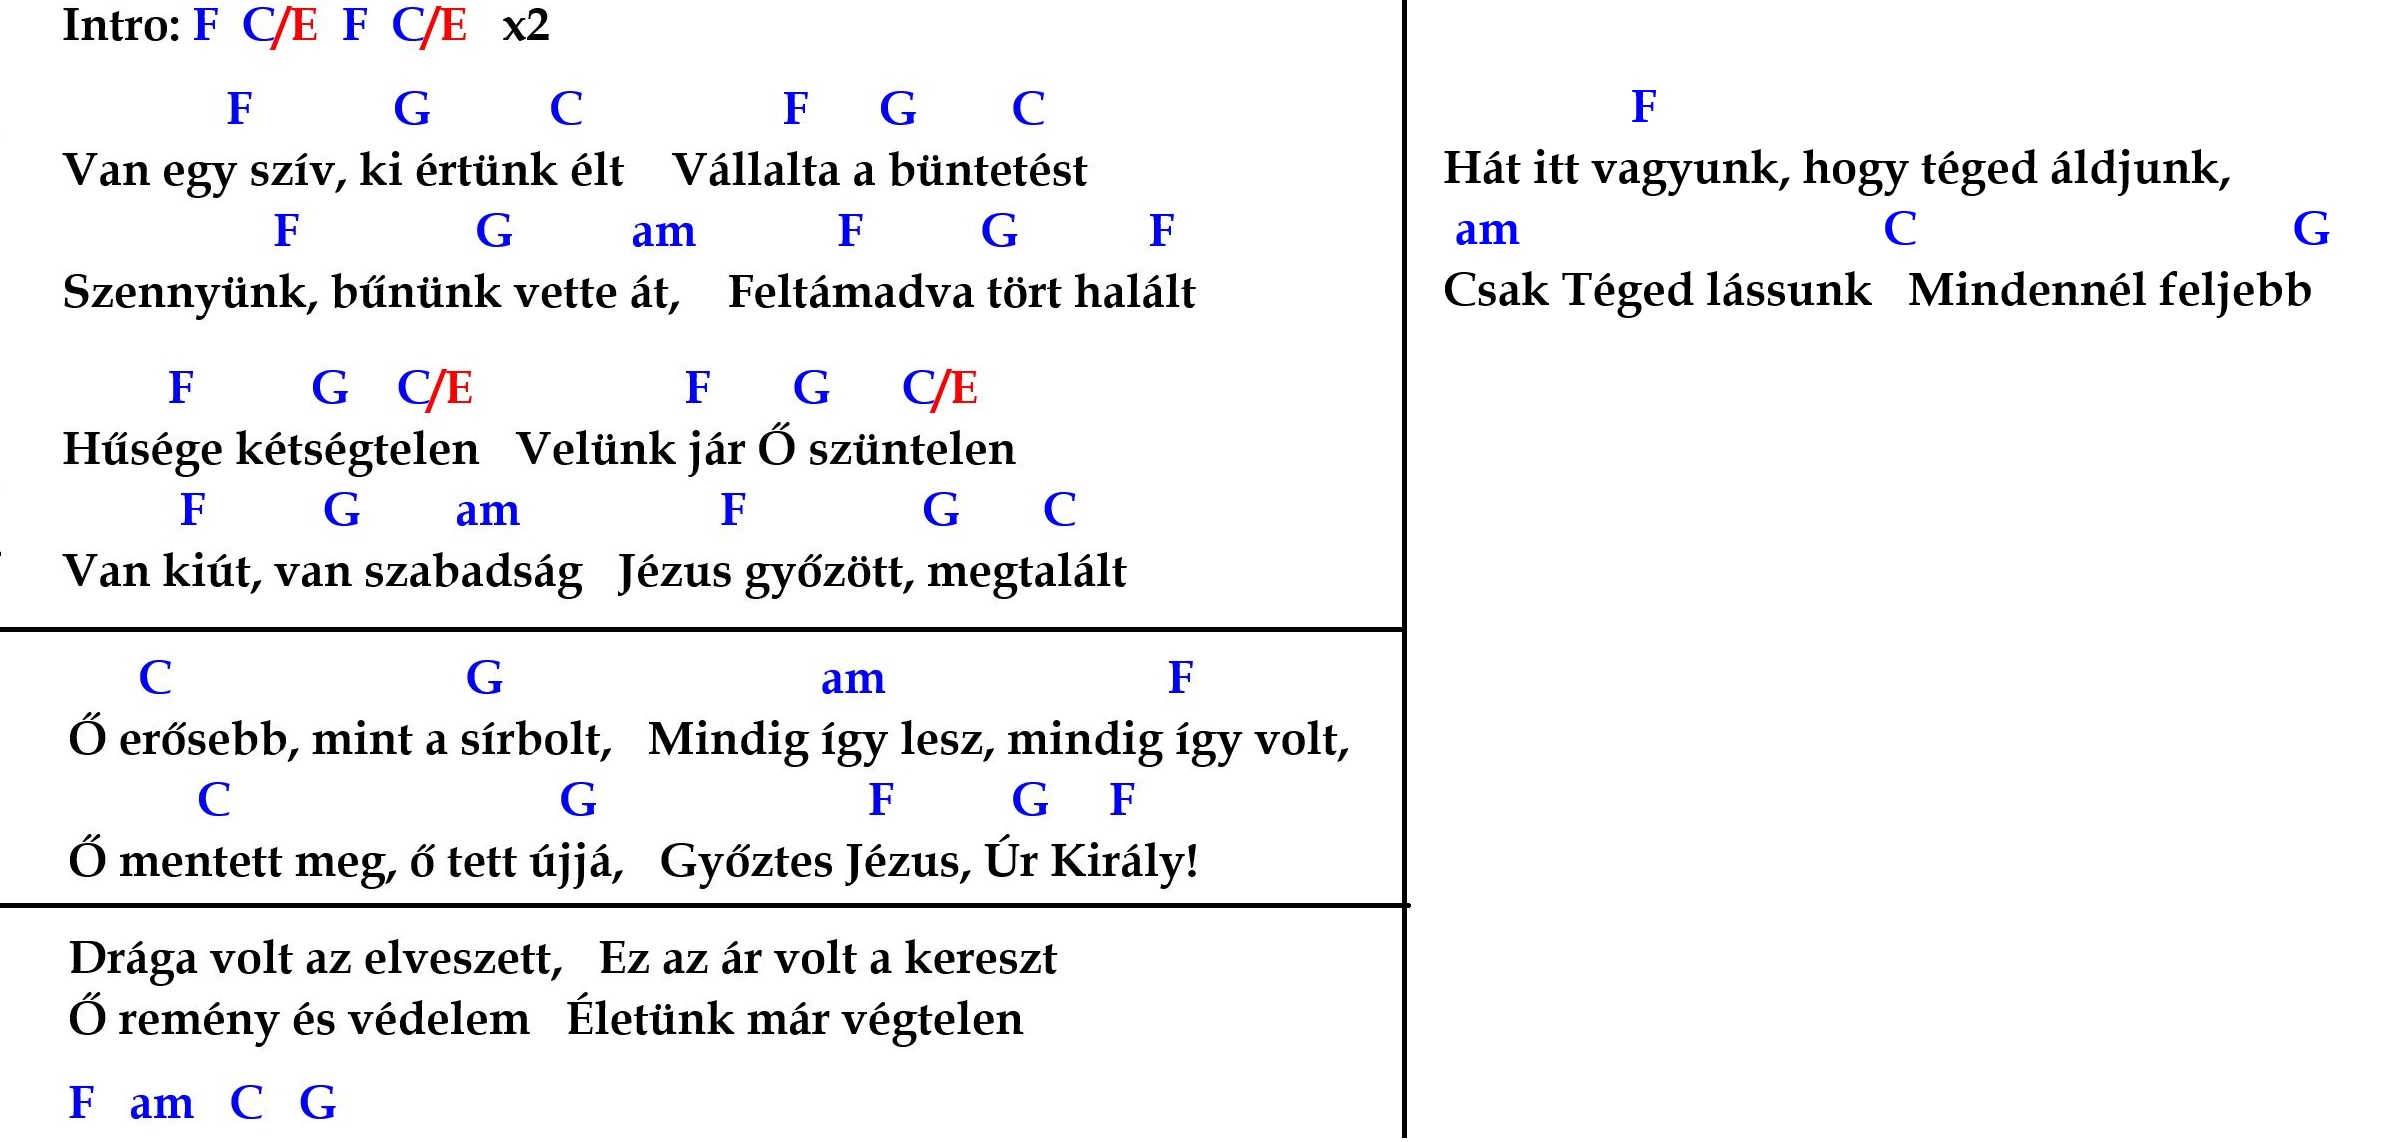
\includegraphics[scale=0.24]{../ImageProcessing/samples/images/Ő erősebb.jpg}
	\caption{Ő erősebb c. dal kottája.}
	\label{fig:Dal1}
\end{figure}

\newpage
Akkor a program megállapítja, hogy ez milyen hangnemben van, az által, hogy milyen akkordok szerepelnek benne a legtöbbször, valamint, a kezdő akkord szerint (viszont most ez megtévesztő, mert F-el kezdődik, miközben a dal C-dúrban van). Mind ez után a felhasználó kiválasztja, hogy milyen hangnembe szeretné lementeni a kottát, tegyük fel, hogy G-dúrban. Ilyenkor az F akkord-hármas C-re, a G D-re, a C G-re és az am em-ra fog változni és így ez a kotta meg lesz G-dúrban. Ahhoz, hogy ez lementhető legyen, ugye vissza kell illeszteni a megfelelő karaktereket a megfelelő színben a képhez, ez a folyamat úgy fog kinézni, hogy a kiválasztott akkordok, mikor szöveggé alakulnak azután el is fognak tűnni a képről, és majd a visszaillesztésnél, a lementett koordináták szerint kerülnek vissza a megfelelő akkordok.